
Mediante la ejecución de los algoritmos en diferentes datasets, se logró observar experimentalmente el funcionamiento de estos y las cualidades que poseen en la práctica. Resulta especialmente interesante destacar aquellos comportamientos que divergen de lo esperado teóricamente. Las pruebas se dividieron en dos grandes testeos: multiplicación de matrices y ordenamiento de datos unidimensionales, cuyos resultados se comentan a continuación.

\begin{itemize}
    \item \textbf{Multiplicación de matrices:}
    Al ejecutar el programa, se obtuvieron los datos retratados en la Tabla \ref{tab:comparativa_matrices}. Información que nos permite ya ver algunos comportamientos inesperados, que son mucho más apreciables si es que se calcula el tiempo promedio ($\bar{T}$) y la memoria promedio ($\bar{M}$) de todos los datos, haciendo uso de las siguientes fórmulas:

    \[ \bar{T} = \frac{1}{k} \sum_{i=1}^{k} t_i \]
    \[ \bar{M} = \frac{1}{k} \sum_{i=1}^{k} m_i \]

    Con estas expresiones, se consolidó la información presentada en la Tabla 2:

    \begin{table}[H]
    \centering
    \caption{Comparativa de resultados: Datos brutos vs. Promedios}
    \label{tab:comparativa_matrices}
    
    % --- TABLA IZQUIERDA (Muestra de Datos Brutos) ---
    \begin{minipage}[t]{0.48\textwidth}
        \centering
        \small
        \begin{tabular}{|l|c|r|c|}
            \hline
            \textbf{Algoritmo} & \textbf{$n$} & \textbf{Tiempo ($s$)} & \textbf{Mem ($KB$)} \\ \hline
            naive & 1024 & 1.87985 & 15872 \\ \hline
            strassen & 1024 & 51.50330 & 45440 \\ \hline
            naive & 256 & 0.01133 & 4352 \\ \hline
            strassen & 256 & 1.02331 & 6272 \\ \hline
            naive & 64 & 0.00034 & 3584 \\ \hline
            strassen & 64 & 0.02053 & 3712 \\ \hline
            naive & 16 & 7.54e-06 & 3456 \\ \hline
            strassen & 16 & 0.00045 & 3456 \\ \hline
        \end{tabular}
        \subcaption{Muestra de resultados brutos significativos}
    \end{minipage}
    \hfill 
    % --- TABLA DERECHA (Promedios Calculados) ---
    \begin{minipage}[t]{0.48\textwidth}
        \centering
        \small
        \begin{tabular}{|l|c|r|c|}
            \hline
            \textbf{Algoritmo} & \textbf{$n$} & \textbf{$\bar{T}$ ($s$)} & \textbf{$\bar{M}$ ($KB$)} \\ \hline
            naive & 16 & 0.000009 & 3427.56 \\ \hline
            naive & 64 & 0.000178 & 3569.78 \\ \hline
            naive & 256 & 0.011011 & 4302.22 \\ \hline
            naive & 1024 & 1.945440 & 15857.78 \\ \hline
            strassen & 16 & 0.000560 & 3434.67 \\ \hline
            strassen & 64 & 0.020883 & 3697.78 \\ \hline
            strassen & 256 & 1.030509 & 6257.78 \\ \hline
            strassen & 1024 & 50.447661 & 45418.67 \\ \hline
        \end{tabular}
        \subcaption{Tiempos y memoria promedio}
    \end{minipage}
    \end{table}

    \textbf{(En la carpeta} \texttt{code/matrix\_multiplication/data/measurements/results.csv} \textbf{se encuentran los datos extendidos de la tabla 1)}
    \\
    \\
    Como se puede apreciar en las tablas, el tiempo promedio del algoritmo de Strassen es significativamente superior (a veces un poco más de un par de cifras significativas) al algoritmo Naive, lo que sorprende ya que en su tiempo teórico este último es de $O(n^3)$, que es peor que el de Strassen con su $O(n^{2.807})$. Y no solo en tiempo Strassen está siendo peor, también en uso de memoria, llegando a ser casi 3 veces más que su competidora, lo que podría señalar cuál es la razón para que su comportamiento temporal se haya disparado. 
    
    A continuación se dejan unos gráficos comparativos que permiten visualizar de mejor manera el comportamiento de los algoritmos durante los test.

    \begin{figure}[H]
    \centering
    % --- GRÁFICO IZQUIERDO (TIEMPO) ---
    \begin{subfigure}[b]{0.48\textwidth}
        \centering
        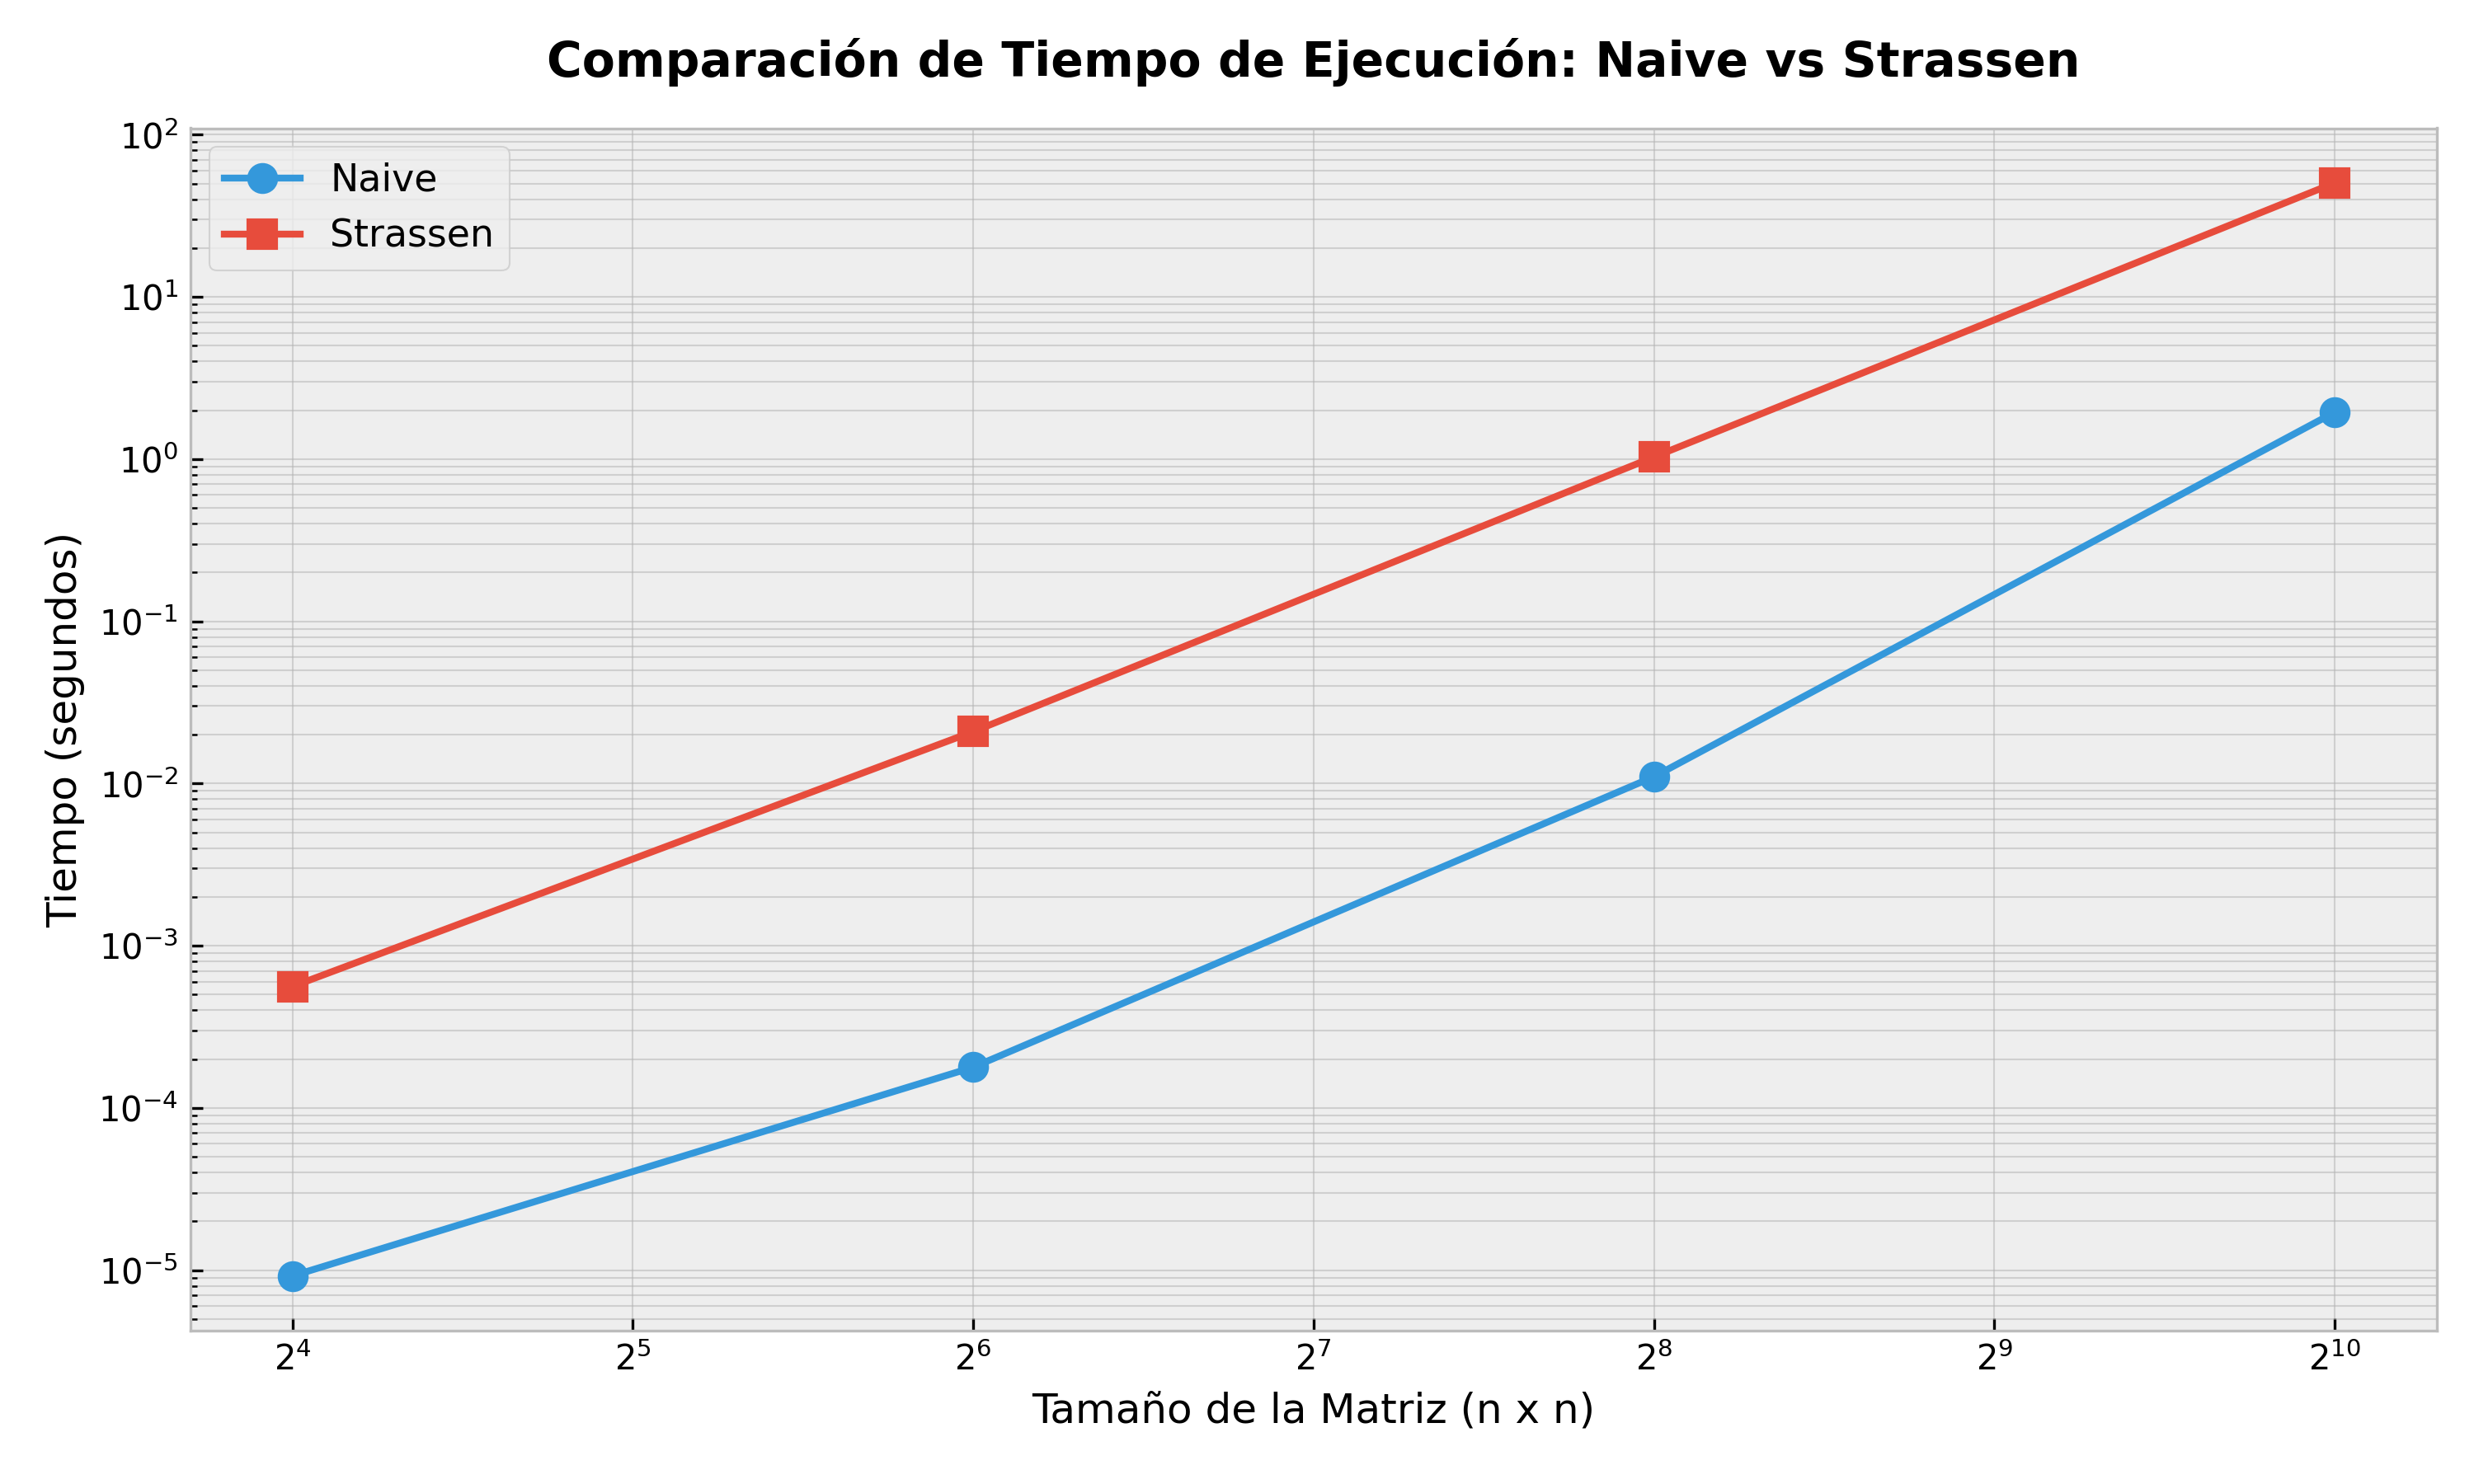
\includegraphics[width=\textwidth]{report/IMG/time_comparison.png}
        \caption{Comparación de tiempo de ejecución.}
        \label{fig:grafico_tiempo}
    \end{subfigure}
    % --- ESTE ESPACIO ES CLAVE ---
    \hfill 
    % -----------------------------
    % --- GRÁFICO DERECHO (MEMORIA) ---
    \begin{subfigure}[b]{0.48\textwidth}
        \centering
        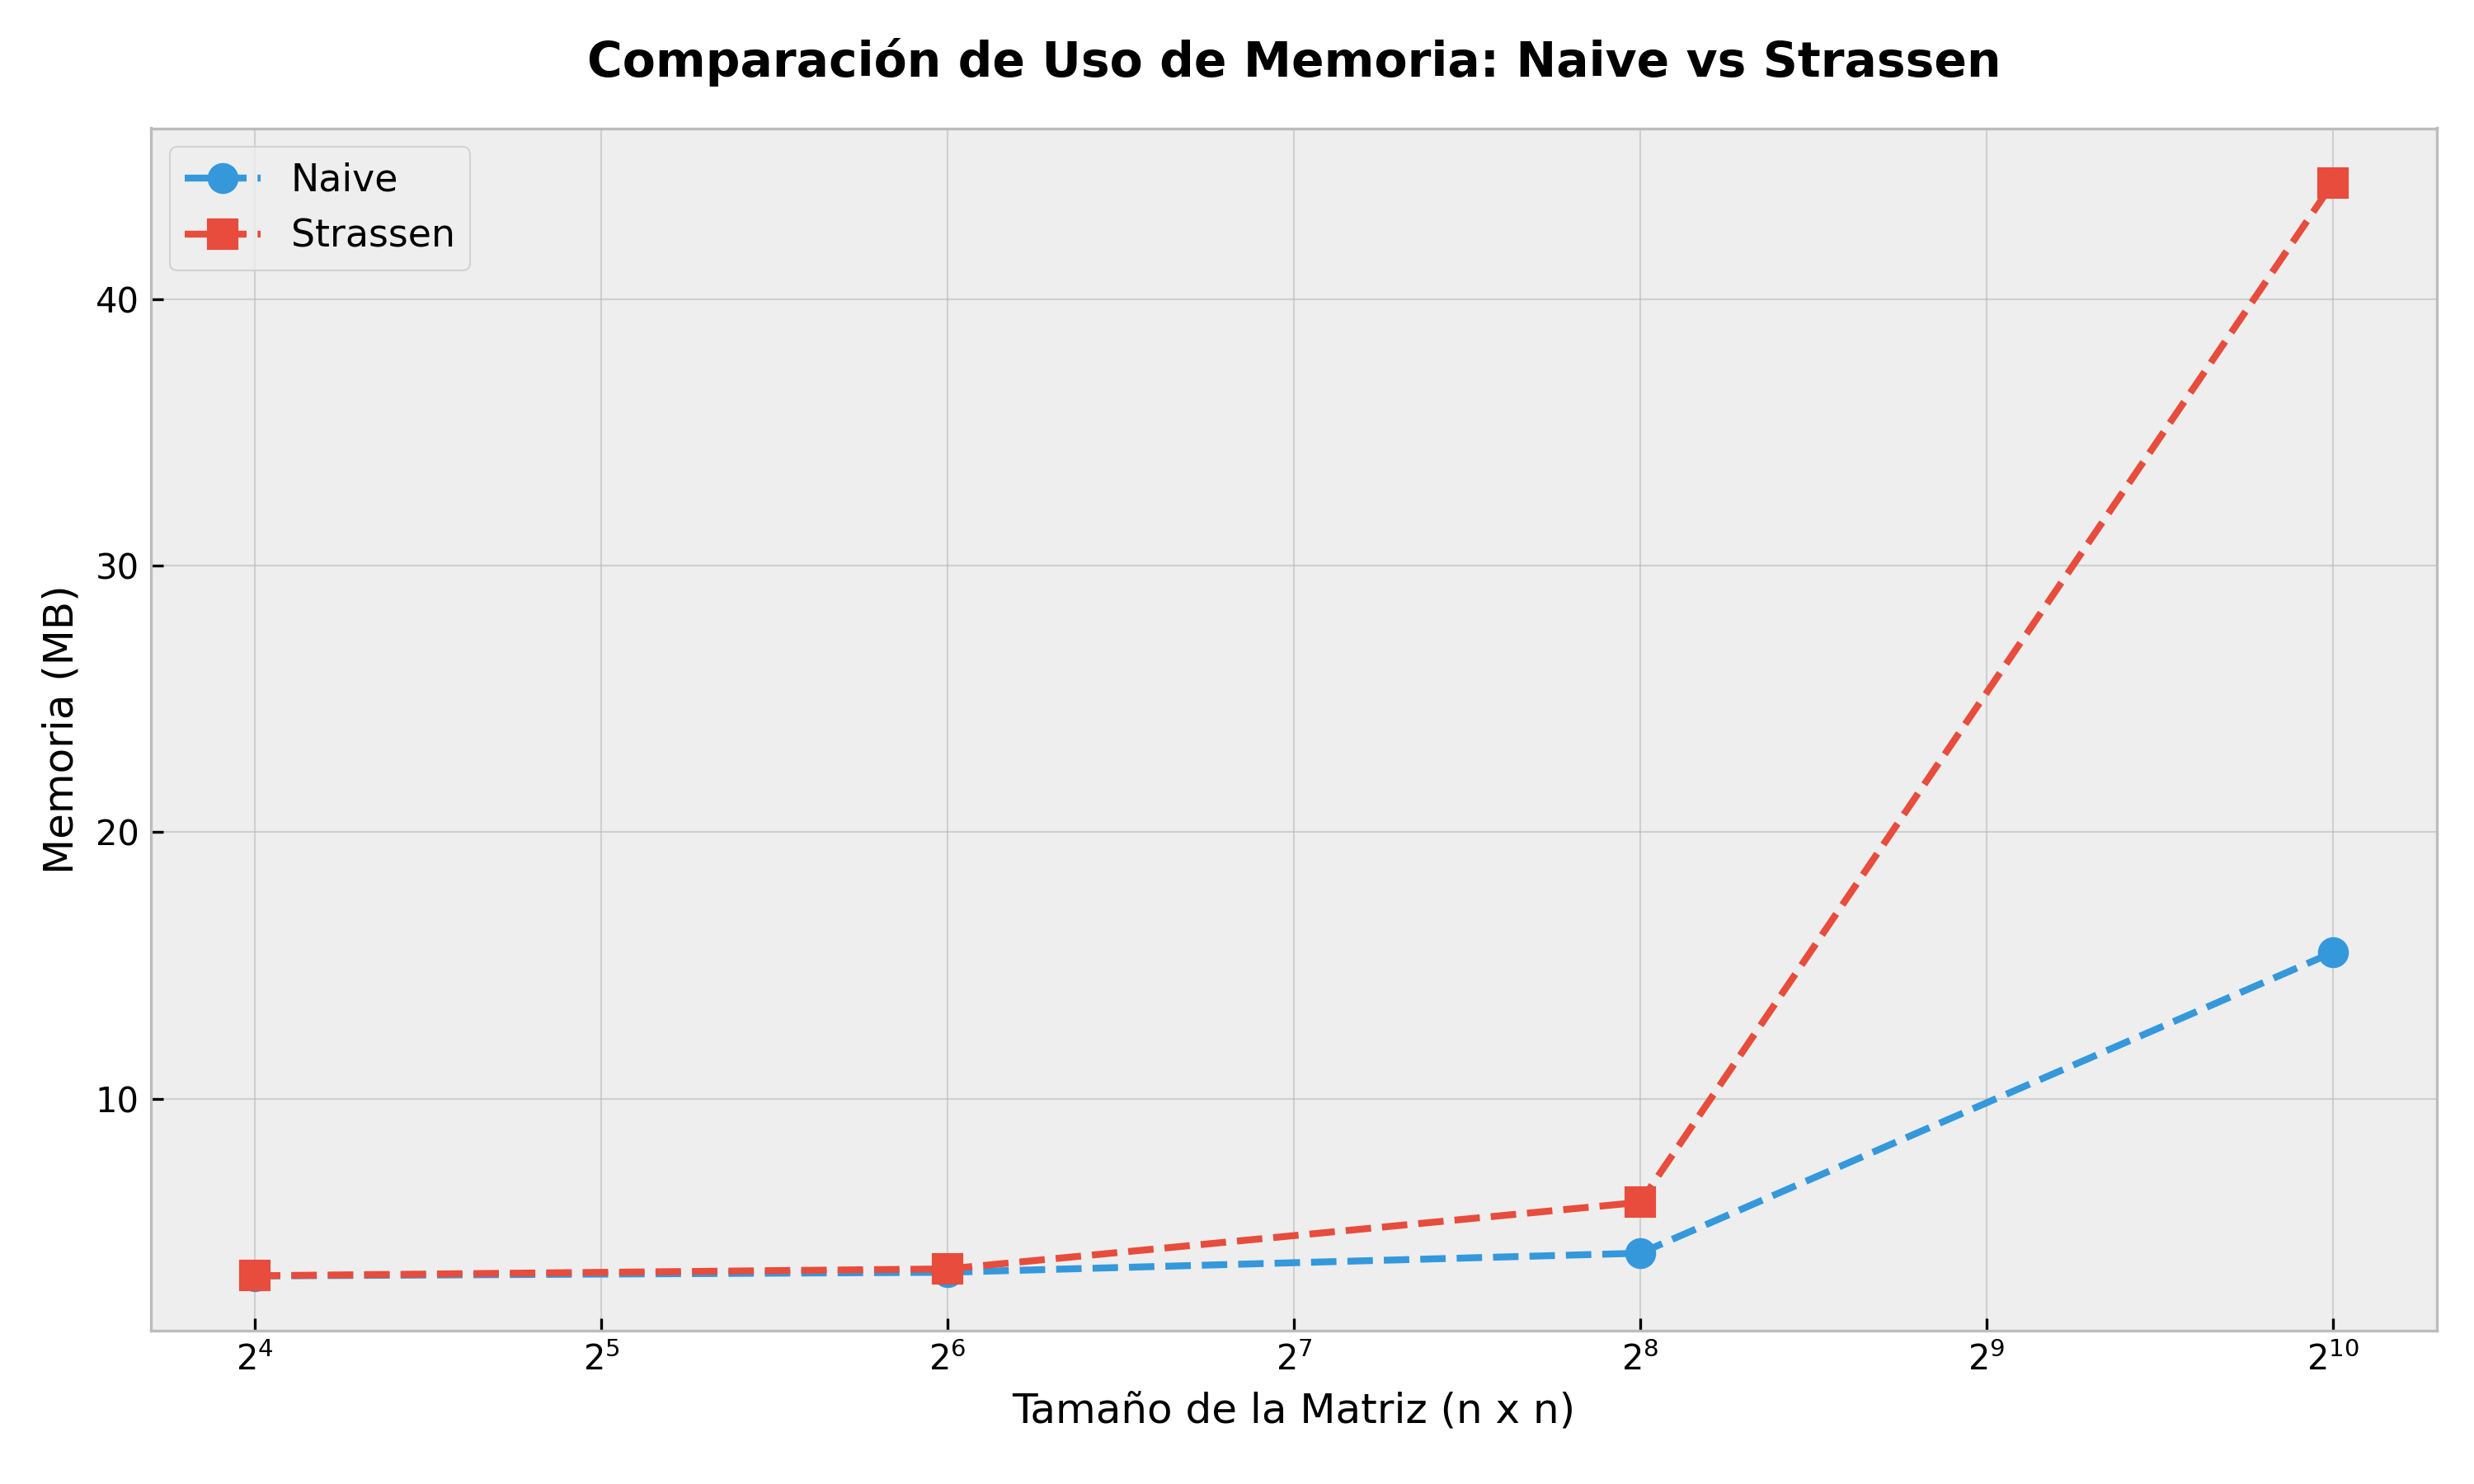
\includegraphics[width=\textwidth]{report/IMG/memory_comparison.png}
        \caption{Comparación de uso máximo de memoria (KB).}
        \label{fig:grafico_memoria}
    \end{subfigure}
    
    % --- LEYENDA PRINCIPAL ---
    \caption{Análisis experimental de complejidad para multiplicación de matrices: Naive vs. Strassen.}
    \label{fig:analisis_experimental}
    \end{figure}

    De estos graficos destaca el abrupto salto de memoria que hace Strassen, esta usando \textbf{3 veces mas memoria} que el algoritmo de Naive y intuitivamente podemos asociar este aumento de consumo a la necesidad de crear  constantemente vectores temporales (p1 a p7) lo que a su vez genera un costo administrativo muy alto que problamente sea lo que este impactando en en el tiempo general del algoritmo. 

    \item \textbf{Ordenamiento de Arreglos Unidimensionales:}
    Para esta etapa se evaluaron los algoritmos MergeSort, QuickSort y el estándar de la librería (\texttt{std::sort}). Las pruebas abarcaron desde $10^1$ hasta $10^7$ elementos, utilizando dominios con pocos duplicados ($D7$) y alta frecuencia de estos ($D1$). Al igual que en las matrices, se aplicaron las fórmulas de promedio para sintetizar la información de desempeño:

    \[ \bar{T} = \frac{1}{k} \sum_{i=1}^{k} t_i \quad ; \quad \bar{M} = \frac{1}{k} \sum_{i=1}^{k} m_i \]

    \begin{table}[H]
    \centering
    \caption{Resultados de Ordenamiento: Comparativa de rendimiento y promedios}
    \label{tab:comparativa_sorting}
    
    % --- TABLA IZQUIERDA (Muestra de Datos Brutos Relevantes) ---
    \begin{minipage}[t]{0.45\textwidth}
        \centering
        \small
        \begin{tabular}{|l|c|r|c|}
            \hline
            \textbf{Algoritmo} & \textbf{$N$} & \textbf{Tiempo ($s$)} & \textbf{Mem ($KB$)} \\ \hline
            stdsort & $10^7$ & 0.24832 & 81624 \\ \hline
            mergesort & $10^7$ & 0.83986 & 81492 \\ \hline
            quicksort & $10^5$ & 4.04266 & 8404 \\ \hline
            stdsort & $10^5$ & 0.00209 & 4312 \\ \hline
            quicksort & $10^3$ & 0.00049 & 3456 \\ \hline
            mergesort & $10$ & 4.74e-06 & 3328 \\ \hline
        \end{tabular}
        \subcaption{Muestra de resultados significativos}
    \end{minipage}
    \hfill 
    % --- TABLA DERECHA (Promedios Calculados de todas las N) ---
    \begin{minipage}[t]{0.52\textwidth}
        \centering
        \small
        \begin{tabular}{|l|c|r|c|}
            \hline
            \textbf{Algoritmo} & \textbf{$N$} & \textbf{$\bar{T}$ ($s$)} & \textbf{$\bar{M}$ ($KB$)} \\ \hline
            stdsort & $10^7$ & 0.27661 & 81597 \\ \hline
            mergesort & $10^7$ & 0.79107 & 81413 \\ \hline
            quicksort & $10^5$ & 2.26443 & 6145 \\ \hline
            stdsort & $10^5$ & 0.00202 & 4310 \\ \hline
            mergesort & $10^5$ & 0.00624 & 4177 \\ \hline
            stdsort & $10^3$ & 2.22e-05 & 3328 \\ \hline
            mergesort & $10^3$ & 6.80e-05 & 3328 \\ \hline
            quicksort & $10^3$ & 2.98e-04 & 3370 \\ \hline
            stdsort & $10^1$ & 5.12e-06 & 3328 \\ \hline
            mergesort & $10^1$ & 6.45e-06 & 3328 \\ \hline
            quicksort & $10^1$ & 5.09e-06 & 3328 \\ \hline
        \end{tabular}
        \subcaption{Tiempos y memoria promedio ($10^1$ a $10^7$)}
    \end{minipage}
    \end{table}

    \textbf{(En la carpeta} \texttt{code/sorting/data/measurements/results.csv} \textbf{se encuentran los datos detallados)}
    \\

    \textbf{Análisis de Fallo Crítico en QuickSort:}
    Un punto fundamental de este test fue la inestabilidad de la implementación manual de QuickSort. Al ejecutar el \texttt{make run}, se obtuvo el siguiente comportamiento en la terminal:

\begin{lstlisting}[language=bash, caption=Log de errores durante la ejecucion de Benchmarks]
Running Benchmarks for 10000000_aleatorio_D1_a...
Segmentation fault (core dumped)
Running Benchmarks for 10000000_ascendente_D1_a...
Segmentation fault (core dumped)
Running Benchmarks for 10000000_descendente_D7_a...
Segmentation fault (core dumped)
\end{lstlisting}

    Este error de \textbf{Segmentation fault} es consecuencia directa de un \textbf{Stack Overflow}. Debido a que el pivote se selecciona como el último elemento (esquema de Lomuto), en arreglos ya ordenados o con dominios pequeños ($D1$), las particiones resultan extremadamente desbalanceadas. Esto provoca que la profundidad de la recursión alcance los $10^7$ niveles, superando el límite de la pila del sistema operativo (8MB), algo que no sucede en \textbf{MergeSort} debido a su división siempre simétrica ($O(\log n)$ en la pila).

    A continuación se presentan los gráficos comparativos de los algoritmos que lograron completar los sets de datos:

    \begin{figure}[H]
    \centering
    \begin{subfigure}[b]{0.48\textwidth}
        \centering
        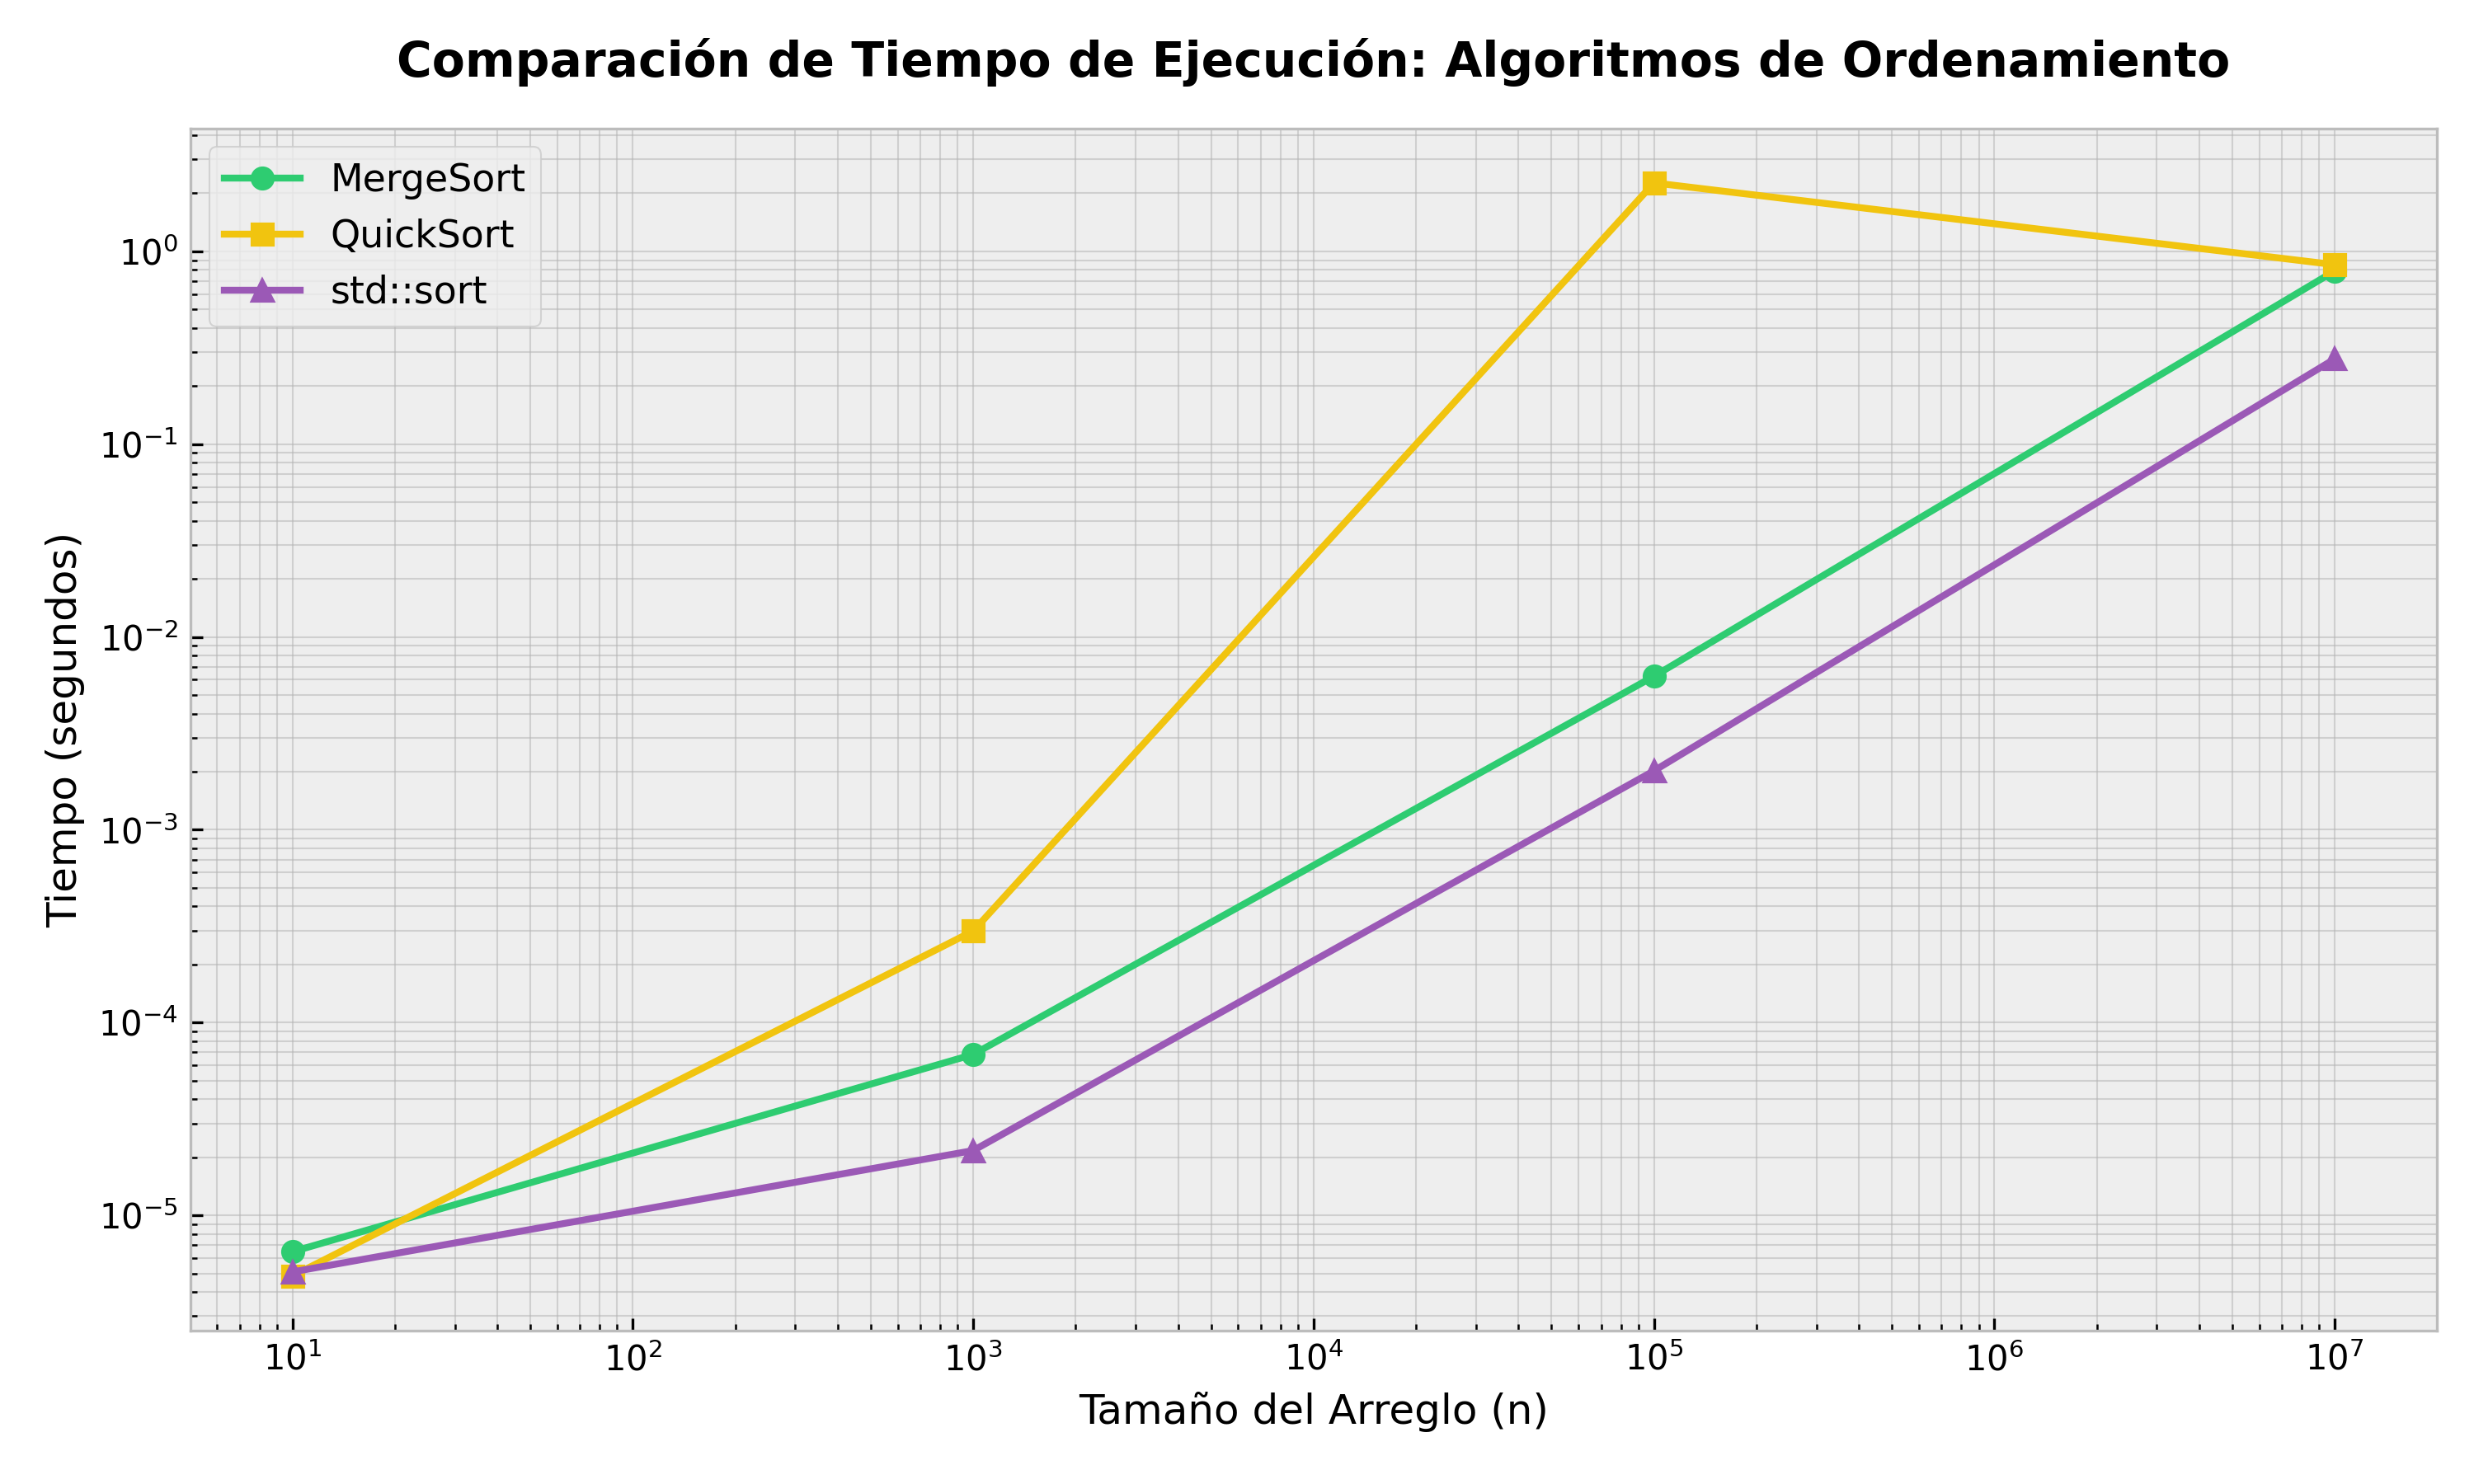
\includegraphics[width=\textwidth]{report/IMG/sorting_time_comparison.png}
        \caption{Tiempo de ejecución}
        \label{fig:sorting_time}
    \end{subfigure}
    \hfill 
    \begin{subfigure}[b]{0.48\textwidth}
        \centering
        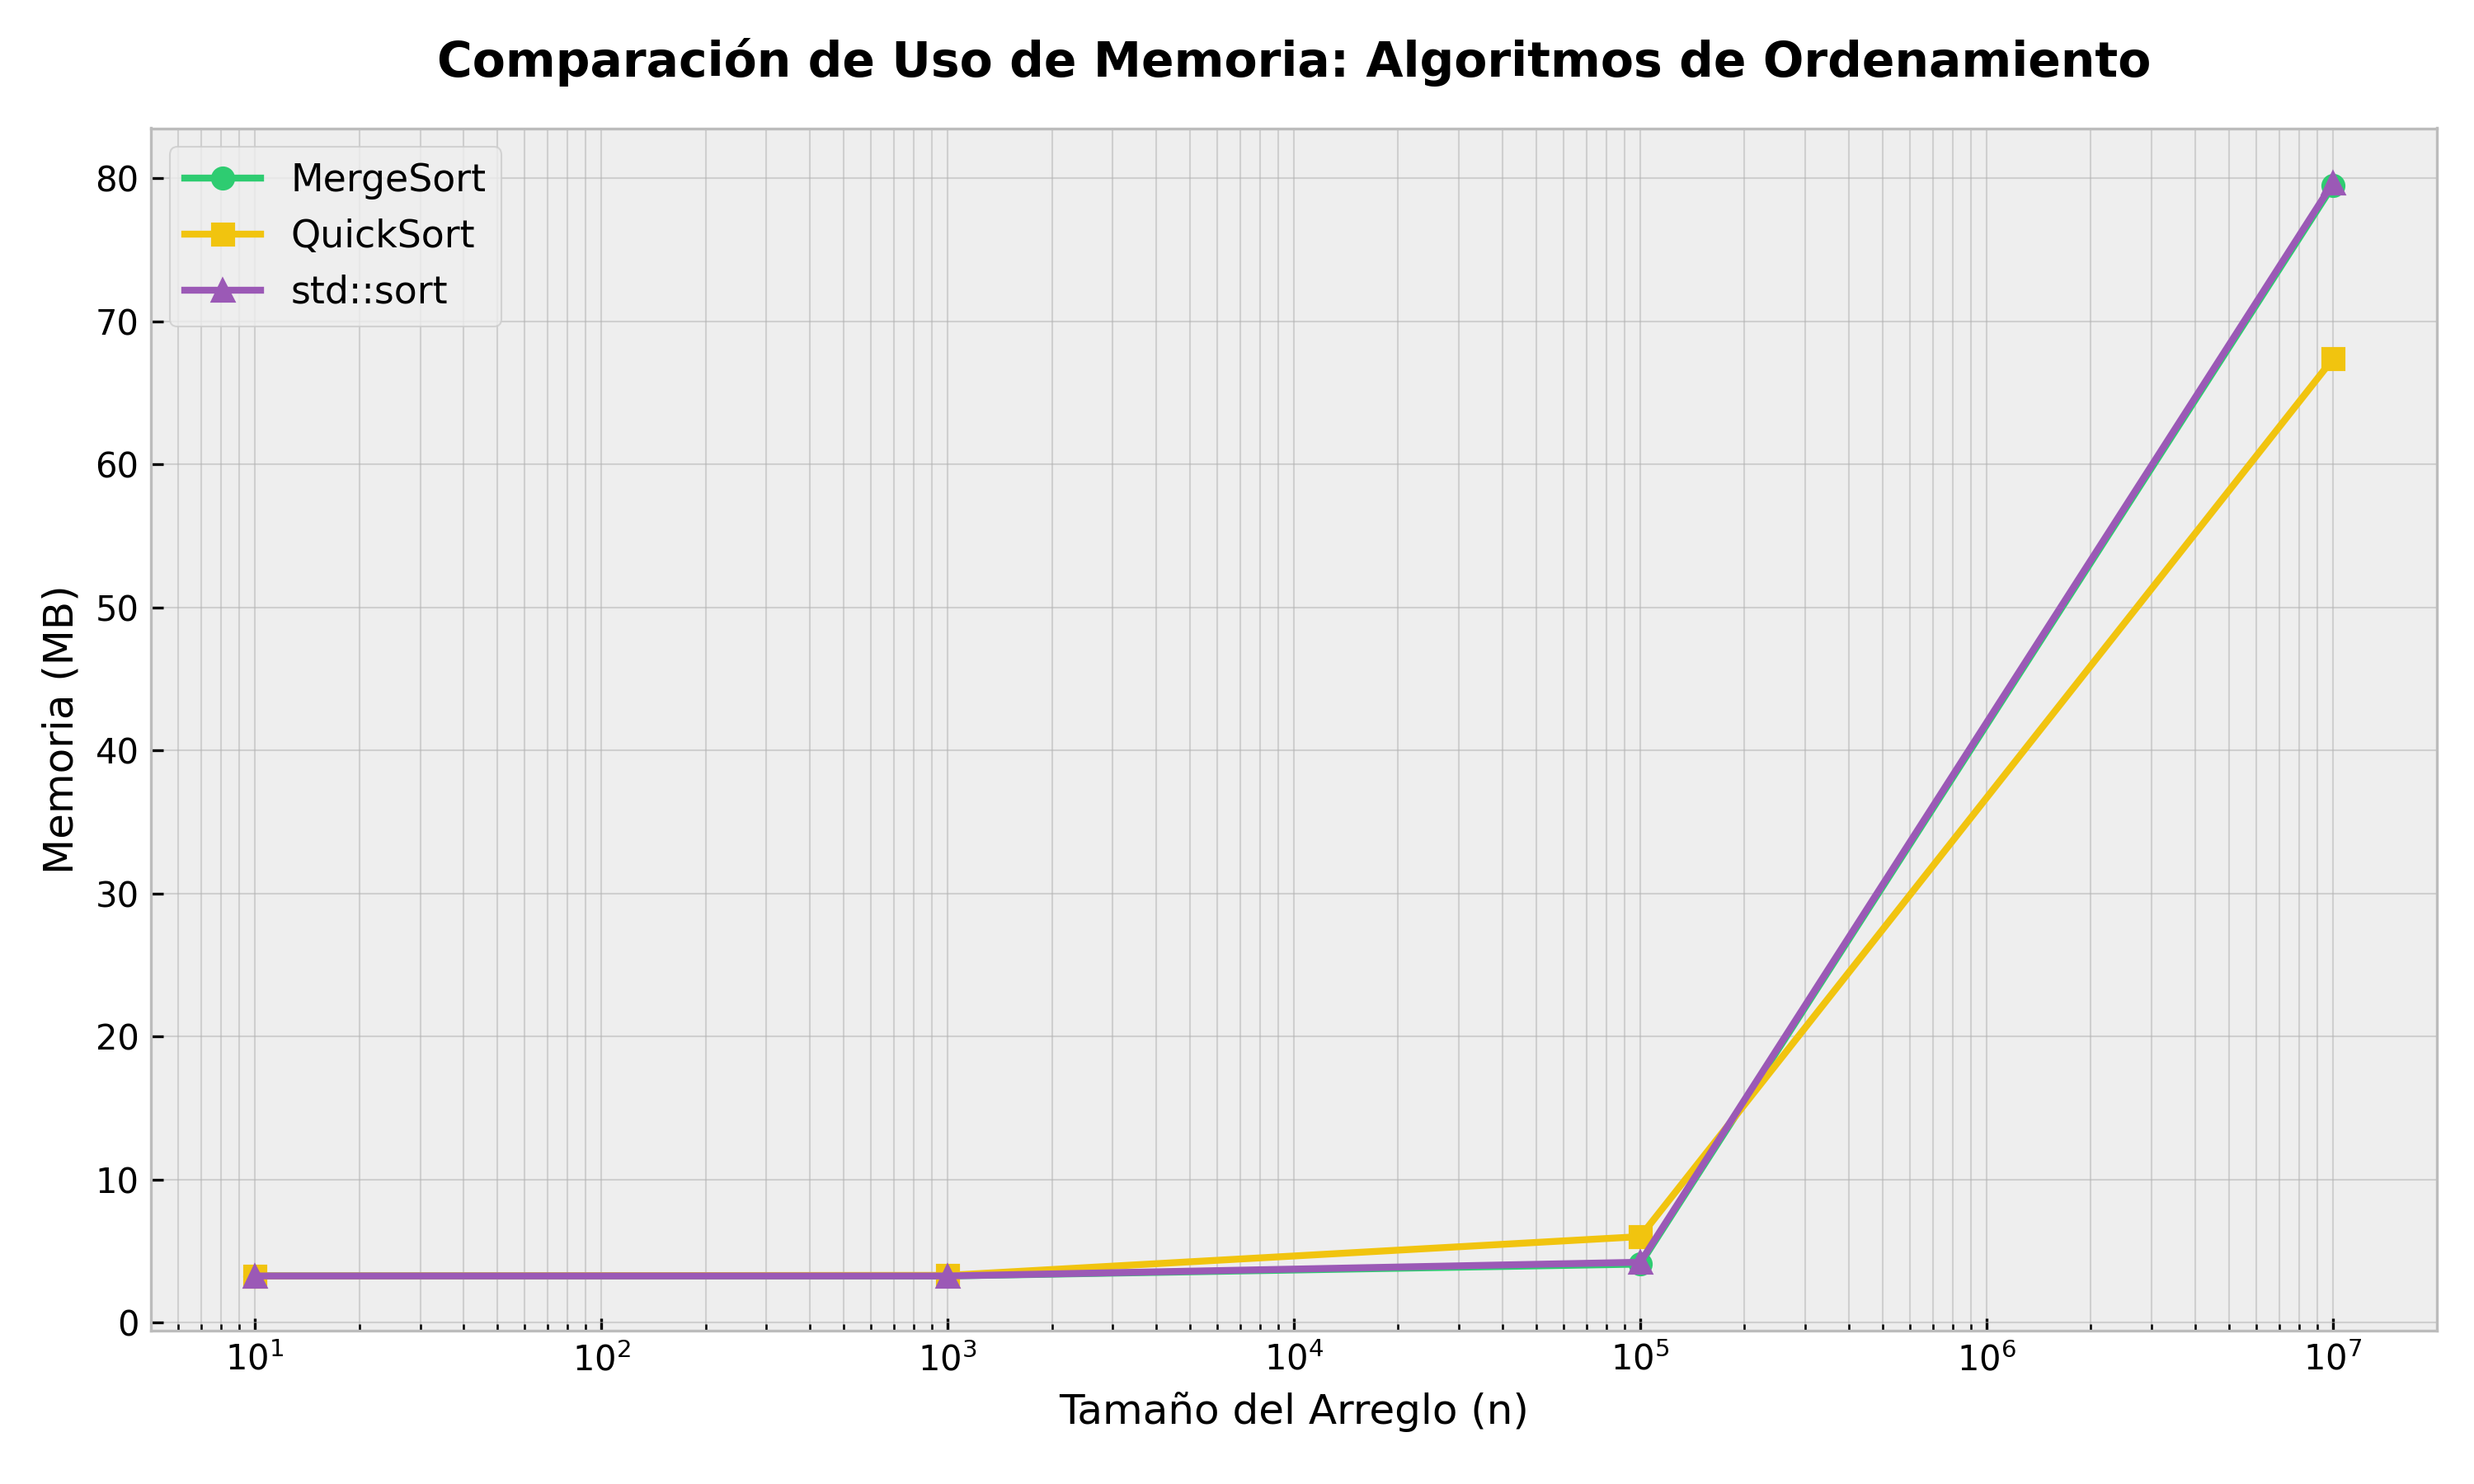
\includegraphics[width=\textwidth]{report/IMG/sorting_memory_comparison.png}
        \caption{Consumo de memoria $O(n)$.}
        \label{fig:sorting_memory}
    \end{subfigure}
    \caption{Análisis experimental de ordenamiento: MergeSort vs. QuickSort vs. Introsort.}
    \end{figure}

    Finalmente, destaca el desempeño de \textbf{std::sort}, el cual implementa \textbf{Introsort}. Este algoritmo es superior porque combina la rapidez de QuickSort con la seguridad de HeapSort (al que cambia si la recursión es muy profunda) y la eficiencia de Insertion Sort para tramos pequeños. Esto explica por qué \texttt{stdsort} es casi 4 veces más rápido que MergeSort y no falla ante los casos que colapsaron a nuestra implementación de QuickSort.
    
\end{itemize}